\begin{table}[H]
\centering
\caption{Puck statistics after filtering. Homogeneity is the mean fraction of a bead's $k$ nearest spatial neighbours that share its NMFreg label, over all beads (k=5, 15, 30) and over germ-cell beads only (k=15).}
\label{tab:homog}
\small
\begin{tabular}{lrrrrrrr}
\toprule
Puck & Condition & Beads & Median UMI & Homog. $k$=5 & $k$=15 & $k$=30 & Germ, $k$=15 \\
\midrule
WT1 & WT mouse & 29,178 & 719 & 0.524 & 0.474 & 0.432 & 0.538 \\
WT2 & WT mouse & 29,607 & 782 & 0.524 & 0.470 & 0.426 & 0.533 \\
WT3 & WT mouse & 39,181 & 604 & 0.561 & 0.507 & 0.464 & 0.561 \\
DB1 & \emph{ob/ob} mouse & 25,377 & 797 & 0.484 & 0.426 & 0.385 & 0.485 \\
DB2 & \emph{ob/ob} mouse & 35,629 & 426 & 0.537 & 0.477 & 0.433 & 0.530 \\
DB3 & \emph{ob/ob} mouse & 30,073 & 684 & 0.574 & 0.518 & 0.473 & 0.568 \\
HU1 & human & 30,464 & 602 & 0.362 & 0.336 & 0.316 & 0.380 \\
HU2 & human & 33,389 & 600 & 0.379 & 0.352 & 0.331 & 0.397 \\
\bottomrule
\end{tabular}
\end{table}

\begin{figure}[H]
\centering
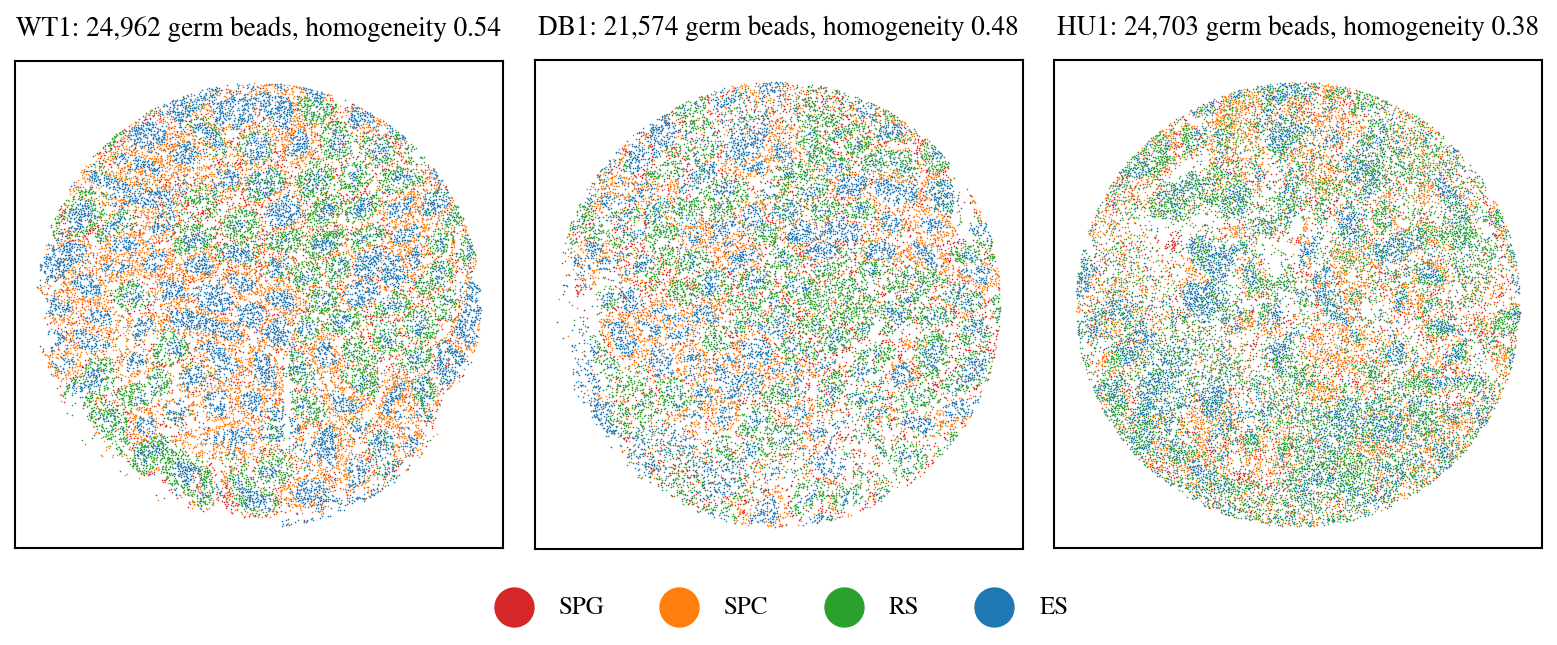
\includegraphics[width=0.95\linewidth]{figs/fig_pucks.png}
\caption{Germ-cell beads of one WT mouse, one \emph{ob/ob} mouse, and one human puck, coloured by NMFreg stage. Tubule cross-sections with a spermatogonia/spermatocyte rim and a spermatid core are visible in mouse; human tubules are larger and stage labels are more mixed.}
\label{fig:pucks}
\end{figure}

\begin{table}[H]
\centering
\caption{Full version of Table~\ref{tab:main}, including the MLP models. Macro-F1, mean $\pm$ SD across test pucks.}
\label{tab:germ4full}
\footnotesize
\setlength{\tabcolsep}{2.5pt}
\begin{tabular}{lcccccc}
\toprule
Model & WT→WT & ob/ob→ob/ob & human→human & WT→ob/ob & WT→human & mouse→human \\
\midrule
LR (expr) & 0.699\,{\scriptsize$\pm$0.013} & 0.717\,{\scriptsize$\pm$0.022} & 0.486\,{\scriptsize$\pm$0.008} & 0.713\,{\scriptsize$\pm$0.026} & 0.385\,{\scriptsize$\pm$0.005} & 0.385\,{\scriptsize$\pm$0.006} \\
LR (expr+nbr) & 0.711\,{\scriptsize$\pm$0.013} & 0.723\,{\scriptsize$\pm$0.016} & 0.513\,{\scriptsize$\pm$0.011} & 0.721\,{\scriptsize$\pm$0.023} & 0.398\,{\scriptsize$\pm$0.007} & 0.396\,{\scriptsize$\pm$0.008} \\
LR (nbr only) & 0.636\,{\scriptsize$\pm$0.003} & 0.607\,{\scriptsize$\pm$0.019} & 0.464\,{\scriptsize$\pm$0.006} & 0.609\,{\scriptsize$\pm$0.029} & 0.365\,{\scriptsize$\pm$0.012} & 0.355\,{\scriptsize$\pm$0.008} \\
LR (expr) + smooth ($\alpha$=0.5) & 0.712\,{\scriptsize$\pm$0.016} & 0.733\,{\scriptsize$\pm$0.019} & 0.501\,{\scriptsize$\pm$0.008} & 0.732\,{\scriptsize$\pm$0.021} & 0.401\,{\scriptsize$\pm$0.005} & 0.400\,{\scriptsize$\pm$0.006} \\
MLP (expr) & 0.693\,{\scriptsize$\pm$0.014} & 0.704\,{\scriptsize$\pm$0.036} & 0.475\,{\scriptsize$\pm$0.012} & 0.704\,{\scriptsize$\pm$0.028} & 0.370\,{\scriptsize$\pm$0.009} & 0.369\,{\scriptsize$\pm$0.009} \\
MLP (expr+nbr) & 0.705\,{\scriptsize$\pm$0.018} & 0.708\,{\scriptsize$\pm$0.029} & 0.498\,{\scriptsize$\pm$0.014} & 0.713\,{\scriptsize$\pm$0.023} & 0.378\,{\scriptsize$\pm$0.013} & 0.375\,{\scriptsize$\pm$0.011} \\
GraphSAGE & 0.711\,{\scriptsize$\pm$0.015} & 0.716\,{\scriptsize$\pm$0.023} & 0.505\,{\scriptsize$\pm$0.013} & 0.721\,{\scriptsize$\pm$0.023} & 0.347\,{\scriptsize$\pm$0.012} & 0.350\,{\scriptsize$\pm$0.012} \\
\bottomrule
\end{tabular}

\end{table}

\begin{figure}[H]
\centering
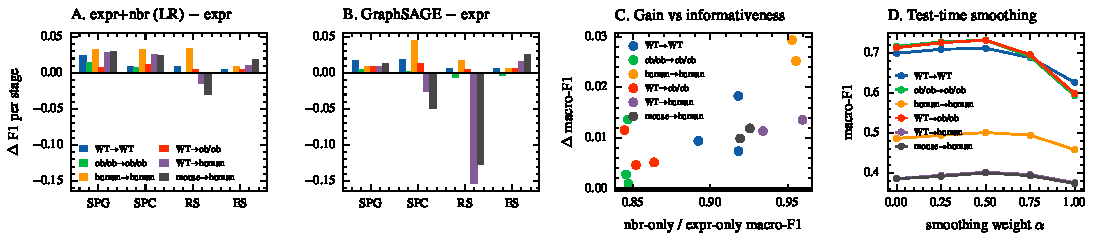
\includegraphics[width=0.8\linewidth]{figs/fig_perclass.pdf}
\caption{(A, B) Per-stage change in F1 from adding spatial context, relative to the expression-only LR, in all six settings; shared vertical scale. (C) Gain from neighbourhood features per test puck against the relative informativeness of context. (D) Test-time smoothing of the expression-only posterior against the weight $\alpha$; $\alpha=1$ replaces each bead's posterior by its neighbours' mean.}
\label{fig:perclass}
\end{figure}

\paragraph{Neighbourhood size and smoothing weight.} Table~\ref{tab:sweeps} reports the LR with neighbourhood features for $k\in\{5,15,30\}$ and test-time smoothing for all $\alpha$.

\begin{table}[H]
\centering
\caption{Sensitivity to neighbourhood size $k$ (LR on expression plus neighbourhood mean) and to the smoothing weight $\alpha$ (expression-only LR posterior smoothed over the test puck's 15-NN graph). Macro-F1 for germ-cell stage, mean over test pucks.}
\label{tab:sweeps}
\small
\begin{tabular}{lccc|ccccc}
\toprule
 & \multicolumn{3}{c|}{expr+nbr, $k$} & \multicolumn{5}{c}{smoothing weight $\alpha$} \\
Setting & 5 & 15 & 30 & 0 & 0.25 & 0.5 & 0.75 & 1 \\
\midrule
WT→WT & 0.715 & 0.711 & 0.708 & 0.699 & 0.709 & 0.712 & 0.689 & 0.626 \\
ob/ob→ob/ob & 0.728 & 0.723 & 0.720 & 0.717 & 0.728 & 0.733 & 0.691 & 0.593 \\
human→human & 0.511 & 0.513 & 0.510 & 0.486 & 0.494 & 0.501 & 0.494 & 0.457 \\
WT→ob/ob & 0.722 & 0.721 & 0.718 & 0.713 & 0.726 & 0.732 & 0.696 & 0.598 \\
WT→human & 0.399 & 0.398 & 0.394 & 0.385 & 0.393 & 0.401 & 0.395 & 0.375 \\
mouse→human & 0.397 & 0.396 & 0.390 & 0.385 & 0.391 & 0.400 & 0.392 & 0.373 \\
\bottomrule
\end{tabular}

\end{table}

\paragraph{Six-class and nine-class labels.} Tables~\ref{tab:coarse6} and \ref{tab:full9} repeat the linear models on all beads with a six-class scheme (four germ stages, tubular somatic, interstitial) and with the original nine NMFreg labels. Macro-F1 is much lower for nine classes because the rare somatic types (endothelial, macrophage, myoid) are near chance from a single bead's expression even in-distribution. The gains from context are smaller than for germ-cell stage (0.4 to 1.0 points within a species for six classes, none for nine classes) but again largest on human in-distribution folds (about two points); across species with nine classes, neither neighbourhood features nor smoothing changes macro-F1 by more than 0.004.

\begin{table}[H]
\centering
\caption{Six-class annotation (SPG, SPC, RS, ES, tubular somatic, interstitial), all beads. Macro-F1, mean $\pm$ SD across test pucks.}
\label{tab:coarse6}
\footnotesize
\setlength{\tabcolsep}{2.5pt}
\begin{tabular}{lcccccc}
\toprule
Model & WT→WT & ob/ob→ob/ob & human→human & WT→ob/ob & WT→human & mouse→human \\
\midrule
LR (expr) & 0.524\,{\scriptsize$\pm$0.018} & 0.549\,{\scriptsize$\pm$0.010} & 0.418\,{\scriptsize$\pm$0.001} & 0.547\,{\scriptsize$\pm$0.009} & 0.301\,{\scriptsize$\pm$0.004} & 0.299\,{\scriptsize$\pm$0.006} \\
LR (expr+nbr) & 0.533\,{\scriptsize$\pm$0.017} & 0.553\,{\scriptsize$\pm$0.007} & 0.441\,{\scriptsize$\pm$0.002} & 0.553\,{\scriptsize$\pm$0.007} & 0.308\,{\scriptsize$\pm$0.003} & 0.306\,{\scriptsize$\pm$0.002} \\
LR (nbr only) & 0.453\,{\scriptsize$\pm$0.003} & 0.429\,{\scriptsize$\pm$0.013} & 0.391\,{\scriptsize$\pm$0.006} & 0.435\,{\scriptsize$\pm$0.017} & 0.280\,{\scriptsize$\pm$0.007} & 0.278\,{\scriptsize$\pm$0.007} \\
LR (expr) + smooth ($\alpha$=0.5) & 0.531\,{\scriptsize$\pm$0.018} & 0.558\,{\scriptsize$\pm$0.016} & 0.433\,{\scriptsize$\pm$0.000} & 0.561\,{\scriptsize$\pm$0.012} & 0.316\,{\scriptsize$\pm$0.006} & 0.315\,{\scriptsize$\pm$0.002} \\
\bottomrule
\end{tabular}

\end{table}

\begin{table}[H]
\centering
\caption{Nine-class annotation with the original NMFreg labels, all beads. Macro-F1, mean $\pm$ SD across test pucks.}
\label{tab:full9}
\footnotesize
\setlength{\tabcolsep}{2.5pt}
\begin{tabular}{lcccccc}
\toprule
Model & WT→WT & ob/ob→ob/ob & human→human & WT→ob/ob & WT→human & mouse→human \\
\midrule
LR (expr) & 0.390\,{\scriptsize$\pm$0.005} & 0.405\,{\scriptsize$\pm$0.000} & 0.309\,{\scriptsize$\pm$0.002} & 0.409\,{\scriptsize$\pm$0.010} & 0.181\,{\scriptsize$\pm$0.006} & 0.182\,{\scriptsize$\pm$0.003} \\
LR (expr+nbr) & 0.392\,{\scriptsize$\pm$0.004} & 0.401\,{\scriptsize$\pm$0.004} & 0.330\,{\scriptsize$\pm$0.001} & 0.413\,{\scriptsize$\pm$0.012} & 0.177\,{\scriptsize$\pm$0.005} & 0.180\,{\scriptsize$\pm$0.004} \\
LR (nbr only) & 0.316\,{\scriptsize$\pm$0.004} & 0.296\,{\scriptsize$\pm$0.010} & 0.280\,{\scriptsize$\pm$0.005} & 0.305\,{\scriptsize$\pm$0.007} & 0.160\,{\scriptsize$\pm$0.006} & 0.168\,{\scriptsize$\pm$0.002} \\
LR (expr) + smooth ($\alpha$=0.5) & 0.393\,{\scriptsize$\pm$0.006} & 0.412\,{\scriptsize$\pm$0.010} & 0.328\,{\scriptsize$\pm$0.001} & 0.416\,{\scriptsize$\pm$0.014} & 0.179\,{\scriptsize$\pm$0.005} & 0.181\,{\scriptsize$\pm$0.003} \\
\bottomrule
\end{tabular}

\end{table}

\paragraph{Gain by sequencing depth and local homogeneity.} Table~\ref{tab:strat} stratifies the accuracy gain from neighbourhood features by the test bead's UMI tertile and by the fraction of its 15 neighbours that share its label. Within a species the gain comes from low-UMI beads; under species shift it comes from high-UMI beads. In every setting context lowers accuracy for beads with heterogeneous neighbourhoods (fewer than 40\% same-label neighbours) and raises it for the rest, so the puck-level gain is a net of these two effects.

\begin{table}[H]
\centering
\caption{Accuracy gain from neighbourhood features (expr+nbr minus expr, LR) stratified by the test bead's UMI tertile within its puck and by its local label homogeneity. Mean over test pucks of each setting.}
\label{tab:strat}
\small
\begin{tabular}{lccc|ccccc}
\toprule
 & \multicolumn{3}{c|}{UMI tertile} & \multicolumn{5}{c}{local homogeneity} \\
Setting & low & mid & high & 0-0.2 & 0.2-0.4 & 0.4-0.6 & 0.6-0.8 & 0.8-1 \\
\midrule
WT→WT & +0.023 & +0.003 & +0.003 & -0.023 & -0.010 & +0.022 & +0.030 & +0.018 \\
ob/ob→ob/ob & +0.015 & -0.001 & -0.002 & -0.036 & -0.011 & +0.017 & +0.024 & +0.019 \\
human→human & +0.047 & +0.021 & +0.018 & -0.048 & +0.014 & +0.091 & +0.111 & +0.089 \\
WT→ob/ob & +0.015 & +0.002 & +0.003 & -0.035 & -0.009 & +0.019 & +0.030 & +0.021 \\
WT→human & -0.011 & +0.002 & +0.029 & +0.000 & -0.007 & +0.011 & +0.034 & +0.050 \\
mouse→human & -0.001 & +0.004 & +0.016 & -0.007 & -0.001 & +0.013 & +0.033 & +0.042 \\
\bottomrule
\end{tabular}

\end{table}

\paragraph{Representation shift.} Table~\ref{tab:shift} reports both measures of how far the feature distribution moves between training and test pucks: the AUC of a logistic regression trained to separate training-domain from test-domain beads, and the per-stage centroid displacement of Fig.~\ref{fig:main}A. Displacement is normalised by the within-class spread in that same space, since averaging over 15 neighbours shrinks the spread as well as the offset; the AUC is not normalised and is reported only to establish that the \emph{ob/ob} condition sits at chance in both spaces.

\begin{table}[H]
\centering
\caption{Representation shift between training and test pucks. Domain-classifier AUC (0.5 = indistinguishable) and mean per-stage centroid displacement in units of within-class spread, for the bead's own embedding and for the neighbourhood mean.}
\label{tab:shift}
\small
\begin{tabular}{llcc|cc}
\toprule
 & & \multicolumn{2}{c|}{domain-classifier AUC} & \multicolumn{2}{c}{centroid shift} \\
Setting & Test & own & nbr & own & nbr \\
\midrule
WT→WT & WT3 & 0.513 & 0.527 & 0.124 & 0.188 \\
WT→ob/ob & DB1 & 0.499 & 0.534 & 0.067 & 0.148 \\
WT→ob/ob & DB2 & 0.503 & 0.518 & 0.091 & 0.189 \\
WT→ob/ob & DB3 & 0.495 & 0.504 & 0.116 & 0.141 \\
WT→human & HU1 & 0.552 & 0.619 & 0.355 & 0.465 \\
WT→human & HU2 & 0.551 & 0.620 & 0.342 & 0.448 \\
\bottomrule
\end{tabular}

\end{table}
